\documentclass[10pt,a4paper]{article}
\usepackage[utf8]{inputenc}
\usepackage{amsmath}
\usepackage{amsfonts}
\usepackage{amssymb}
\usepackage{tikz}
\usetikzlibrary{shapes, positioning, decorations.text}
\begin{document}
\title{Trebuchet}
	\section{Optimum Release Angle}
		At what angle should a projectile be launched to achieve the greatest range?
		If the angle is too large the projectile will go very high but will not have much forward velocity.
		If the angle is too low the projectile will be moving forward very quickly but will not be in the air long enough to make it anywhere.
		What angle will balance these two scenarios and provide the optimum altitude with the best forward velocity?
		Do you have a guess? Think of throwing a ball. What angle do you use when you are trying to really get it to go far?
		Should we use that guess, or can we use our knowledge of math to \emph{prove} what will be the best angle?
		
		\begin{figure}
		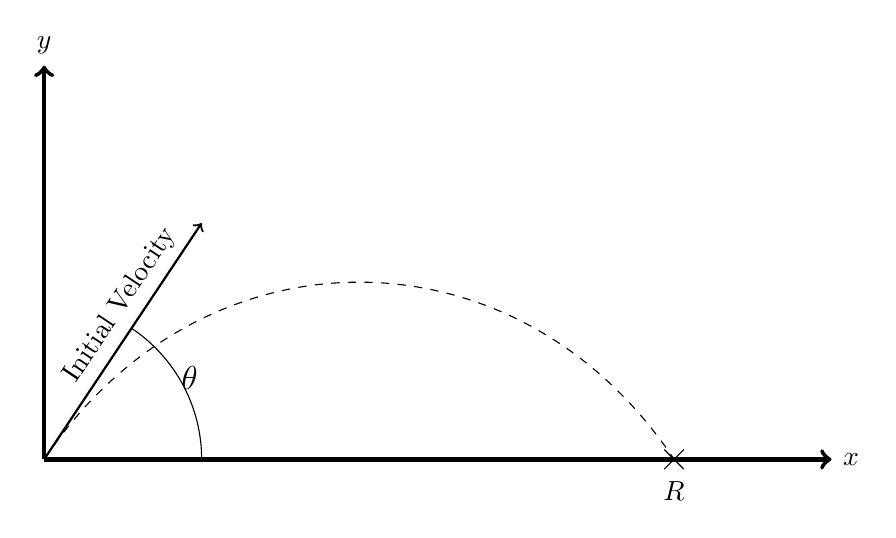
\begin{tikzpicture}
			\draw[style=dashed] (0, 0) .. controls (2,3) and (6,3) .. (8, 0);
			\draw[->,ultra thick] (0,0)--(10,0) node[right]{$x$};
			\draw[->,ultra thick] (0,0)--(0,5) node[above]{$y$};
			\node[cross out, draw] at (8,0) {};
			\draw[->, thick] (0,0) -- (2,3) node[pos=0.6, above, sloped] (TextNode) {Initial Velocity};
			\draw (2,0) arc (0:56:2) node[pos=0.4, above] (TextNode) {\large{$\theta$}};
			\node at (8,-0.4) {$R$};
		\end{tikzpicture}
		\caption{What value of $\theta$ will produce the largest $R$?}
		\label{fig:launchAngle}
		\end{figure}
		
		
\end{document}